\documentclass[12pt]{article}

\usepackage[utf8]{inputenc}
\usepackage{newunicodechar}
\usepackage{float}
\usepackage[utf8]{inputenc}
\usepackage{newunicodechar}
\usepackage{titlesec}
\usepackage{textcomp}
\usepackage{enumitem}
\usepackage{amsmath}
\usepackage{ragged2e}
\usepackage{cancel}
\usepackage{titling}
\usepackage{amssymb}
\usepackage[margin=1.5cm, lmargin=2.5cm]{geometry}

\usepackage{tikz}
\usepackage{graphicx}
\usepackage{caption}
\usepackage{pythonhighlight}
\graphicspath{ {./images/} }
\newcommand*\circled[1]{\tikz[baseline=(char.base)]{
            \node[shape=circle,draw,inner sep=2pt] (char) {#1};}}
\newcommand{\ans}[1]{\boldsymbol{\underline{#1}}}
\newcommand{\textans}[1]{\textbf{\underline{#1}}}
\newcommand{\vm}[1]{\begin{vmatrix}#1\end{vmatrix}}
\newcommand{\vb}[1]{\begin{bmatrix}#1\end{bmatrix}}
\newcommand{\m}[1]{\mathbb{#1}}
% \newcommand{\suct}[3]{\chapter{\textbf{#1} #2}#3}
\newcommand{\enum}[1]{\begin{enumerate}[label=\alph*)]#1\end{enumerate}}
\newcommand{\numenum}[1]{\begin{enumerate}[label=\arabic*.]#1\end{enumerate}}

\DeclareRobustCommand{\[}{\begin{equation}}
\DeclareRobustCommand{\]}{\end{equation}}

\usepackage{setspace}
\setlength{\parindent}{1cm}
\onehalfspace

\usepackage{fontspec}
 
\setmainfont[SizeFeatures={Size=14}]{Times New Roman}
\numberwithin{equation}{section}
\counterwithin{figure}{subsection}

\title{Kinodynamic Motion Planning}
\author{}



\begin{document}
\maketitle

\section{Abstract}

Autonomous navigation systems usually include a path planner and a local planner.
The first one provides a somewhat kinematically reasonable path, which often cannot be passed by a robot,
while the second one tries to adapt the path to the dynamic environment and other constraints that were not checked by the path planner.
This work is an attempt to create an optimized RRT-based path planner that takes into account nonholonomic constraints.
This is achieved through an analysis and combination of already existing solutions, usage of R-Trees, techniques like goal-biased sampling and more. As a result, open source reference implementation in Python constructs trees that require far less local (reactive) planning than typically.
\subsection{Keywords}{}{}\hfill

Path planning, Collision avoidance, Nonholonomic constraints, Rapidly exploring Random Tree, R-Tree, Reeds-Shepp Car.

\section{Introduction}

Motion planning and autonomous vehicles have been developing for quite long time already and in recent 20 years those areas have grown
from enterprise-only solutions (i.e. robotic arms and other manufacturing devices) to consumer-friendly ones (robot vacuums and "autopilots" in cars).
If initially the problem was to "get from point A to point B", by this time it has been expanded with operation in dynamic environments, collision avoidance, computation efficiency and others.

All of the mentioned problems have one thing in common - Configuration Spaces framework that is used to describe the
state of the robot in the environment. In order to state the problem one should define C-Space - $\mathcal{C}$, which includes configurations of the robot $q$, world $\mathcal{W}$ (including obstacles) and other constraints.

This work is aimed to solve the problem of planar path-planning, thus $\mathcal{W}=\mathbb{R}^2$. Some parts of the world are occupied by the obstacles $\mathcal{O}\subset\mathcal{W}$ defined by polygons, which cannot be self-intersecting. And finally the robot - a rigid body $\mathcal{A}$,
which can translate in the world, making $\mathcal{C}$ a manifold $M_1=\mathbb{R}^2$, and rotate around its bounding box center, which adds $M_2=\mathbb{S}^1$, thus without obstacles:
\[
\mathcal{C}=\mathbb{R}^2\times\mathbb{S}^1=SE(2)
\]

The robot's configuration in the space is defined as a vector $q=(x,y,\theta)$ and the space that it is occupying as $\mathcal{A}(q)\subset\mathcal{W}$.
Thus, the configuration space for obstacles is:
\[
\mathcal{C}_{obs}=\{q\in\mathcal{C}\mid\mathcal{A}(q)\cap\mathcal{O}\neq\emptyset \}
\]
\[
\mathcal{C}_{free}=\mathcal{C}\setminus\mathcal{C}_{obs}
\]

The algorithm is created with holonomic - the robot can only travel in $\mathcal{C}_{free}$ - and nonholonomic constraints in mind - it uses Reeds-Shepp Car model and steering function as the only way to produce a path from $q_1\in\mathcal{C}_{free}$ to $q_2\in\mathcal{C}_{free}$, making some configurations in $C_{free}$ unreachable. The Reeds-Shepp Car has only two gears - forward and reverse ($u\in\{-1,1\}$); and angular velocity that depends on maximum turning radius with unit-velocity $r_{turn}$ - $w = \frac{v=1}{r_{turn}}$. In general, the path would be a non-linear function of time, as a turn is a curve. However, in order for a robot to be able to follow the path, each turn is approximated with a given level of discretization $\delta$ to a set of straight lines:

\[
\begin{cases}
\dot{x}=x_{prev} + u\cdot\delta\cdot\cos{\theta}\\
\dot{y}=y_{prev} + u\cdot\delta\cdot\sin{\theta}\\
\dot{\theta}=\theta_{prev}+u\cdot \frac{\delta}{r_{turn}}
\end{cases}
\]

Finally, the starting points are defined as $q_i\in\mathcal{C}_{free}$ and the goal point is $q_g\in\mathcal{C}_{free}$. The local planner should produce a path, which is a set of connected linearized curves that were provided by the steering function.

Generally, industry solves such problem with either a "sampling" algorithm (RRT and variants, PRM) or a graph traversal algorithm like A*. Right now RRT-like algorithms are used more as with a proper set of improvements they can converge quite fast. The data on obstacles is often stored as points in KD-Tree and the collision detection is performed by querying it. Nonholonomic constraints are usually left to the reactive planner. There are several
drawbacks related to those approaches. Firstly, the use of KD-Tree implies a complexity increase on tree expansion, as KD-Tree is not meant to be updated. Secondly, collision detection in such cases is often done by checking the area of some radius around the robot, which makes it impossible for a planner to create a path through narrow corridors, or by checking its bounding box, which is inefficient for any shape except for rectangles that are aligned to the axes (which is not true for any rotated rectangle). And finally, lack of nonholonomic constraints might make the whole path unreachable. The aim of the presented algorithm is not to suffer from those issues with as little overhead compared to others as possible.
This is achieved with the help of R*-Tree, special polygon approximation technique, goal-biased sampling and nearest neighbor randomization.

\section{Literature Overview}

All previous conclusions about "the industry" were obtained by analysing recent researches published under IEEE, ICRA, IROS and other robotics-related conferences.

\section{The Proposed Method}
Our method is based on the RRT algorithm and essentially is an extension for it. The difference from other works lies in data structures,
point sampling approach and collision detection.

\subsection{Sampling}

By default, RRT algorithm picks a random point $q\in\mathcal{C}_{free}$ and tries to build a trajectory from the nearest point in the tree to it (at the first iteration the
nearest point is set to be $q_i$).
The way to determine that the point is reachable is usually constructing a straight line between the sample point and the existing one.
Then, if trajectory is built, the point is added the tree.

A common enhancement to this process is goal-biased sampling. In this case, with a parameterized probability instead of choosing a random point in $C_{free}$. This approach, however,
has a flaw. If the tree has grown close to the $q_g$ with only one branch with last node $q_1$ and due to nonholomonic constraints cannot reach the $q_g$, all later samples that
were changed on $q_g$ will get trapped by $q_1$, which has minimal distance to the $q_g$. Until a new point $q_2: dist(q_2, q_g) < dist(q_1, q_g)$ is added to the tree.
In order to increase the chances of "untrapping" the $q_g$, we propose the following: since after sampling a point or choosing the $q_g$ as the sample point the algorithm tries to 
find the nearest nodes already added to the tree, one could select a random node from the set of n-closest nodes without any computational drawback. 

\begin{figure}
\begin{center}
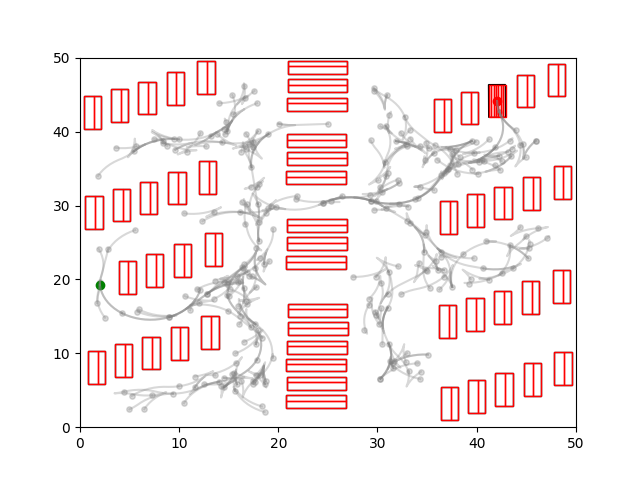
\includegraphics[scale=0.7]{images/car_trapped.png}
\captionsetup{width=0.6\textwidth}
\caption{An example of a vehicle nonholonomically trapped due to angular precision. It stands at the finish point in the wrong direction.}
\end{center}
\end{figure}

Additionally, instead of computing Euclidean distances to all nodes, our algorithm will query the R-Tree on the closest neighbors and compute the Reeds-Shepp distance to them. 

\subsection{Tree and obstacles in R-Tree}

As the data structure for the tree points we propose R-Tree, which does not always require full tree rebuild for an insertion.
While R-Tree does not drastically differ in complexity terms from a KD-Tree, it has an advantage of being able to store not just vertices,
but spatial data in forms of rectangles.

Some works proposed the use of R-Trees as a structure for obstacles as well. However, in shaped that is not a rectangle and not perfectly aligned to the axes requires significantly
more $\mathcal{C}_{free}$ space than it actually should.

\section{Performance analysis}

\subsection{Sample options}

The next step was to find optimal value for sample options parameter. It stands for the number of neighbours that RTree algorithm picks from when creating a new sample. The algorithm was tested on 4 values for sample options parameter (1, 3, 6, 10) and 12 different start and end obstacles configurations with sample size equal to 60. That is overall sample size is equal to 2880.

\begin{figure}[H]
\begin{center}
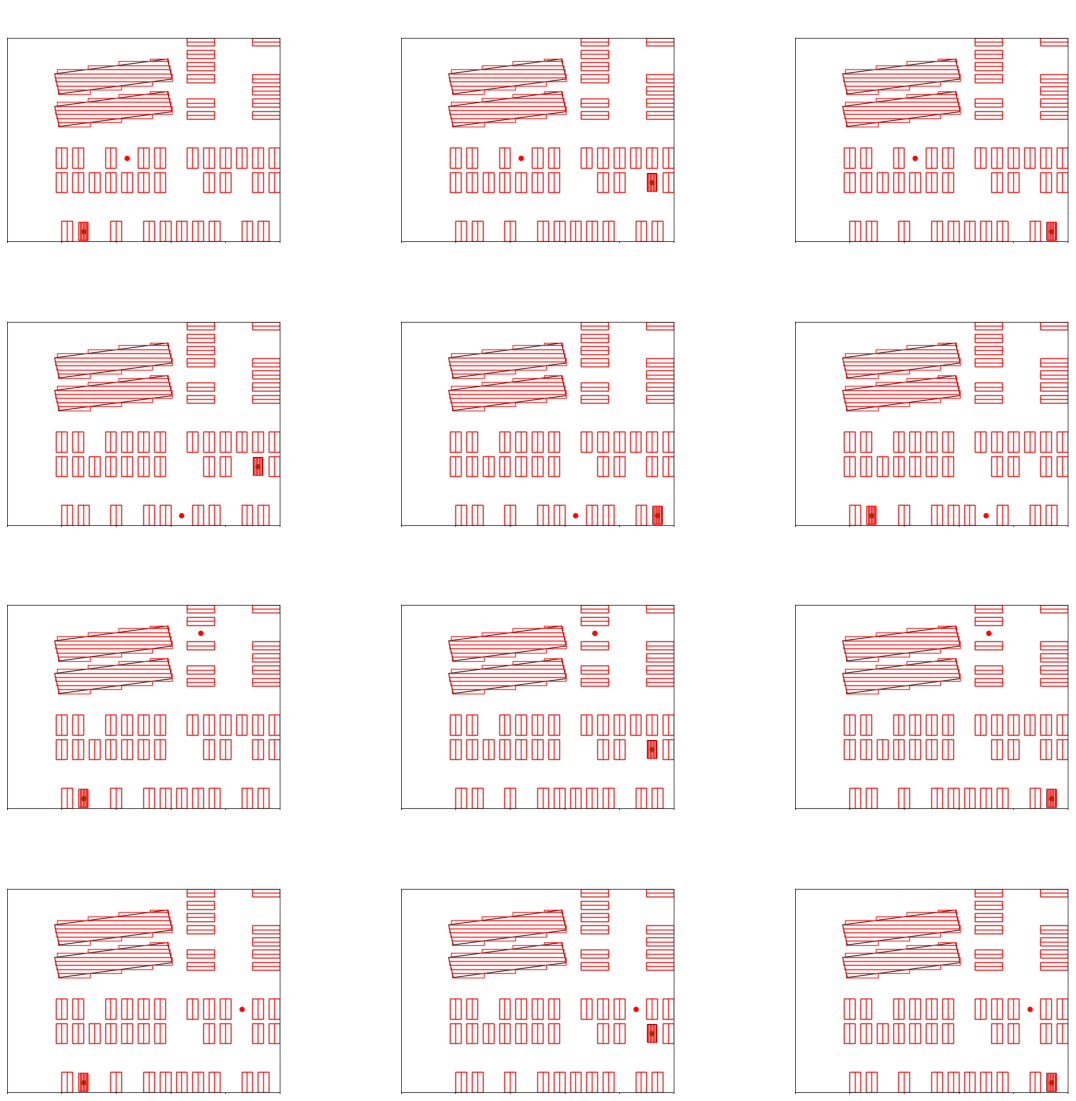
\includegraphics[scale=0.4]{images/12positions.png}
\captionsetup{width=0.6\textwidth}
\caption{12 start-end configurations selected for testing. Starting point is marked by a colored red car with a green dot, ending point is marked by a red dot.}
\end{center}
\end{figure}

Depending on the sample options value, the following plots were generated.

\begin{figure}[H]
\begin{center}
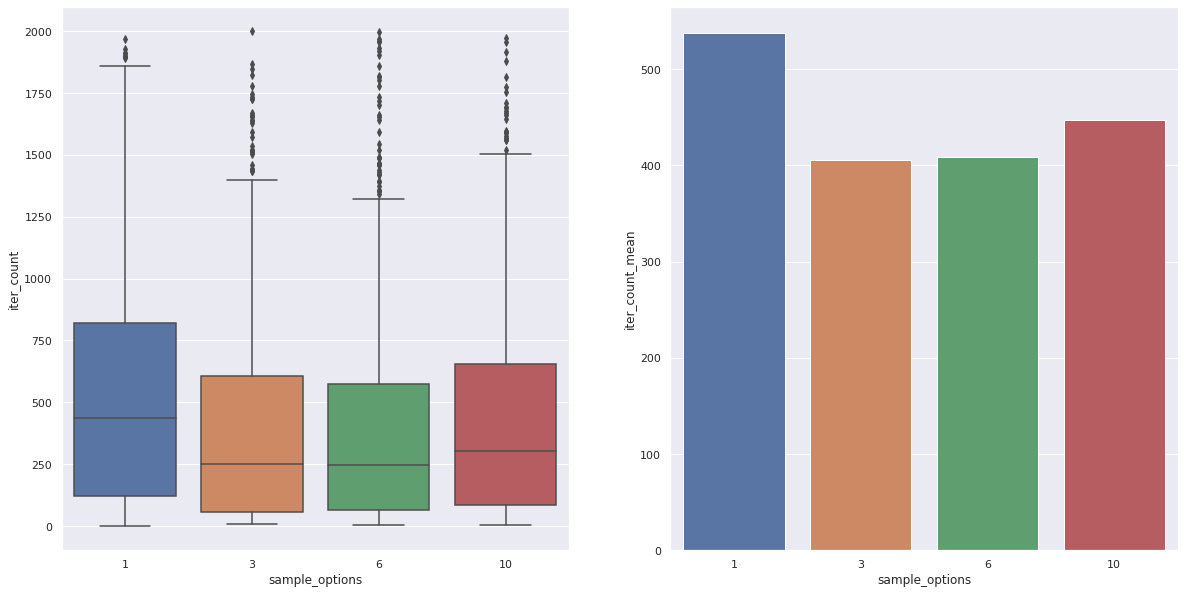
\includegraphics[scale=0.4]{images/so_iter_count.png}
\captionsetup{width=0.6\textwidth}
\caption{Distribution of number of iterations per each value of sample options.}
\end{center}
\end{figure}

Figure 5.1.2 suggests that the parameter has effect on the number of iterations the algorithm executes. The box plot (left) shows that the number of iterations tends to decrease when the number of samples is approximately between 3 and 6 (inclusive). Although the number of outliers is greater for these values than for others, this does not imply worse performance. The bar plot (right) confirms that assumption, representing the mean iterations count.

\begin{figure}[H]
\begin{center}
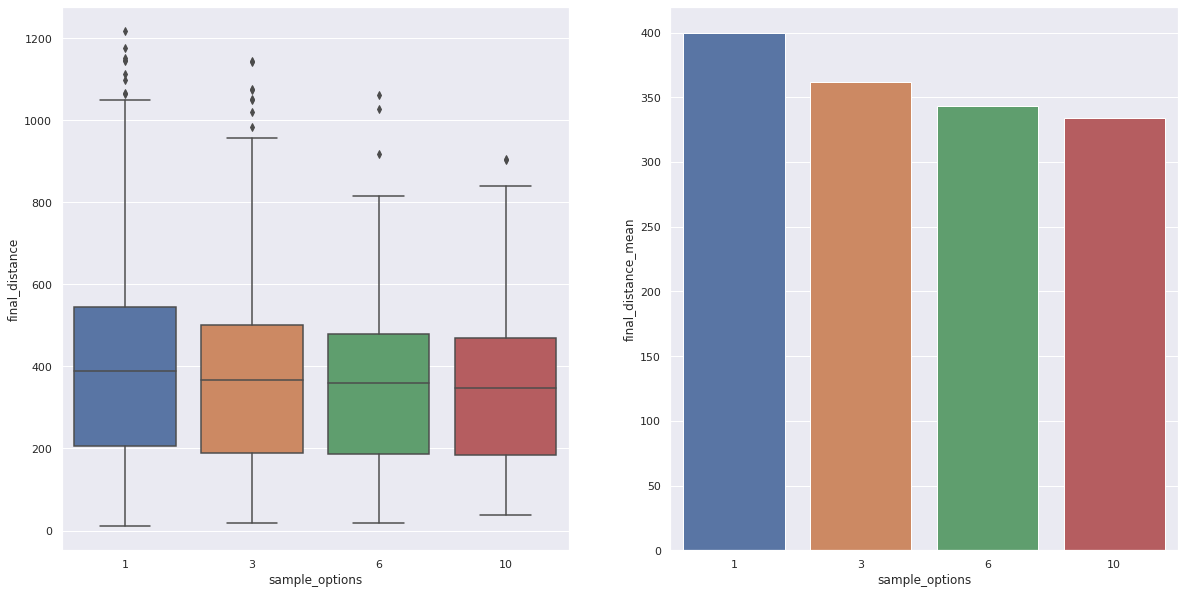
\includegraphics[scale=0.4]{images/so_final_distance.png}
\captionsetup{width=0.6\textwidth}
\caption{Distribution of final distance of a path generated by the algorithm per each value of sample options.}
\end{center}
\end{figure}

Figure 5.1.3 suggest a negative trend for final distance for increasing number of options. One possible explanation is that cardinality of options set allows RRT to create longer edges which eventually results in total distance decrease, while smaller edges often create more winding paths.

\begin{figure}[H]
\begin{center}
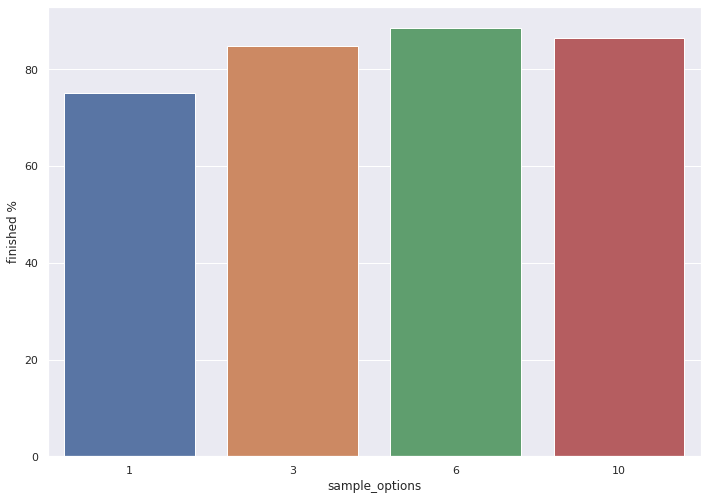
\includegraphics[scale=0.4]{images/so_finished.png}
\captionsetup{width=0.6\textwidth}
\caption{Distribution of convergence percentage of the algorithm per each value of sample options.}
\end{center}
\end{figure}

Figure 5.1.4 suggest that the sample options value has effect on the convergence rate. Similar to Figure 5.1.2 values close to 6 yield best performance.

Thus, the algorithm performance depends on the cardinality of options set. More precisely, algorithm performance peaks for parameter values close to 6.

\subsection{Start and finish points configurations}

Next, a subset containing observations with sample option parameter set to 6 was examined. The start and finish points configurations were categorized as short, medium and long based on the mean final distance. Categories are presented in Figure 5.2.1, Figure 5.2.2 and Figure 5.2.3.

\begin{figure}[H]
\begin{center}
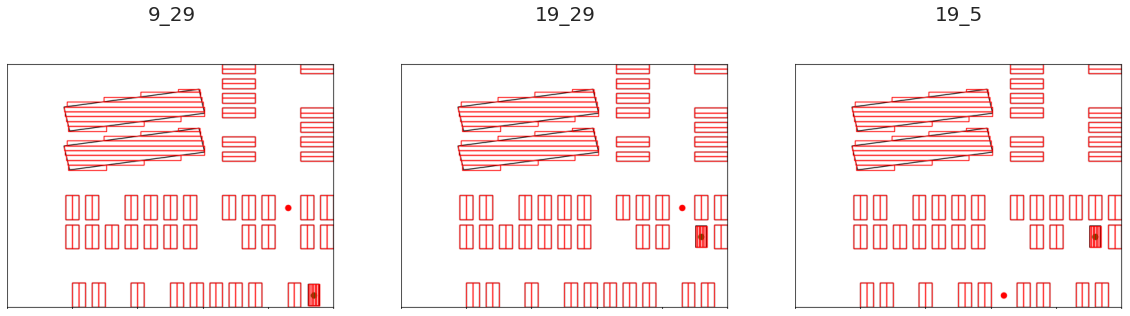
\includegraphics[scale=0.4]{images/shorts.png}
\captionsetup{width=0.6\textwidth}
\caption{Start/end configurations categorized as short.}
\end{center}
\end{figure}

\begin{figure}[H]
\begin{center}
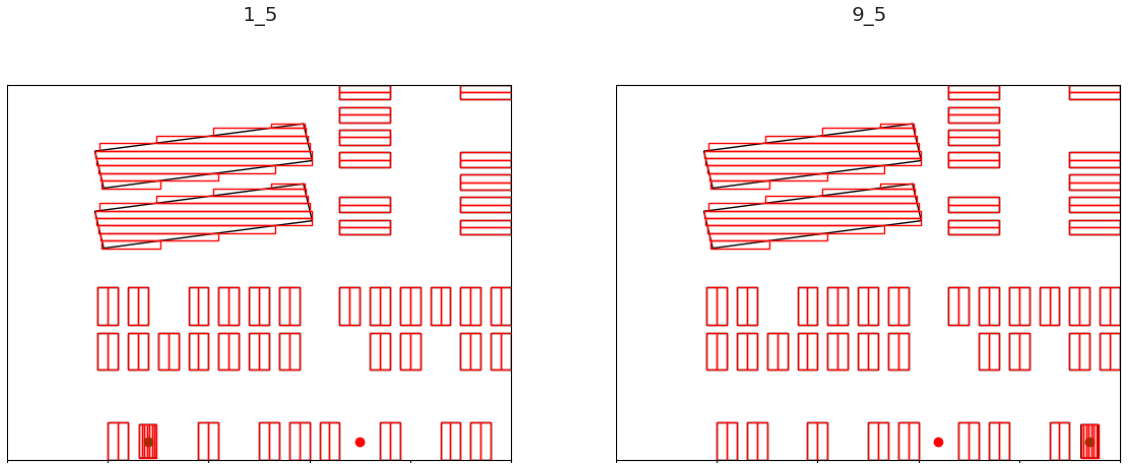
\includegraphics[scale=0.4]{images/mediums.png}
\captionsetup{width=0.6\textwidth}
\caption{Start/end configurations categorized as medium.}
\end{center}
\end{figure}

\begin{figure}[H]
\begin{center}
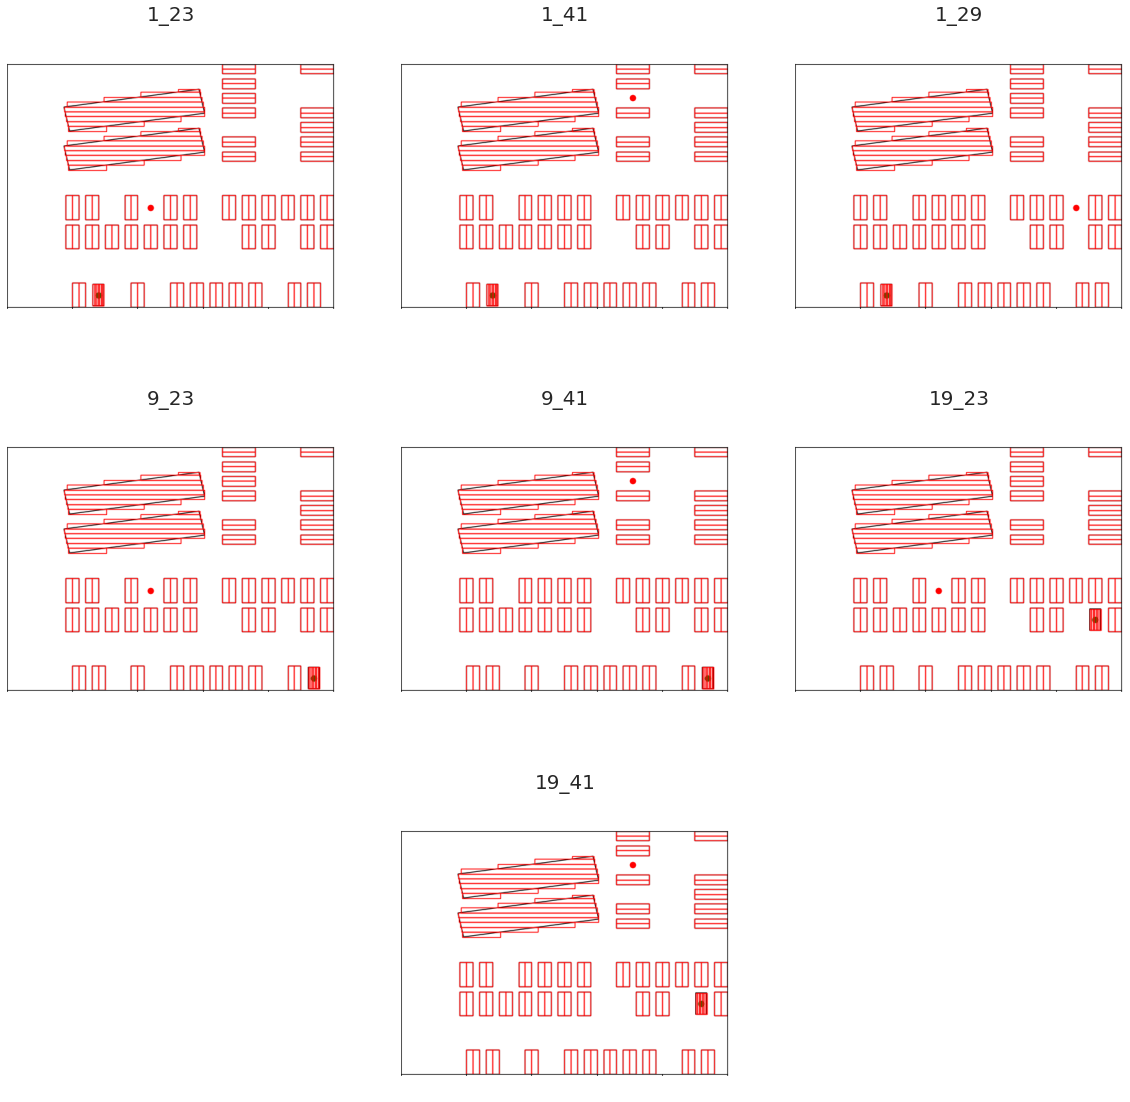
\includegraphics[scale=0.4]{images/longs.png}
\captionsetup{width=0.6\textwidth}
\caption{Start/end configurations categorized as long.}
\end{center}
\end{figure}

The algorithm showed a score of 100\% convergence rate on short and medium distances. The average convergence rate for long distances is approximately 80\%, although this parameter varies significantly among configurations of this type. More detailed data is presented in Figure 5.2.4.

\begin{figure}[H]
\begin{center}
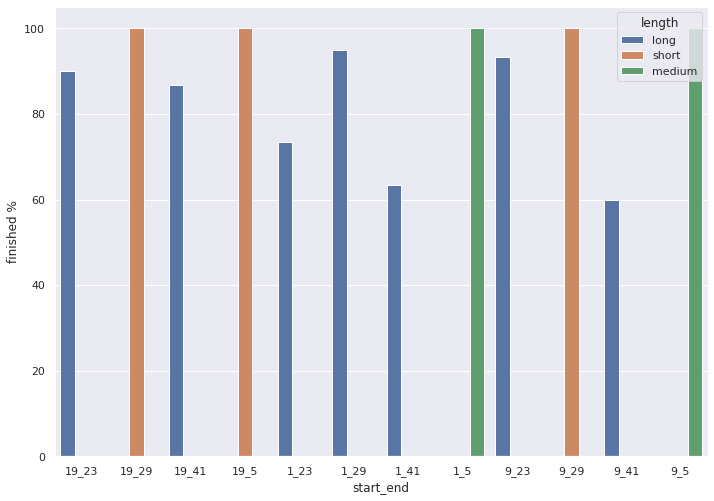
\includegraphics[scale=0.5]{images/se_finished.png}
\captionsetup{width=0.6\textwidth}
\caption{Convergence rate depending on start/end configurations.}
\end{center}
\end{figure}

The average number of iterations highly depends on the distance category, as expected. As Figure 5.2.5 suggests long paths require significantly more iterations to converge.

\begin{figure}[H]
\begin{center}
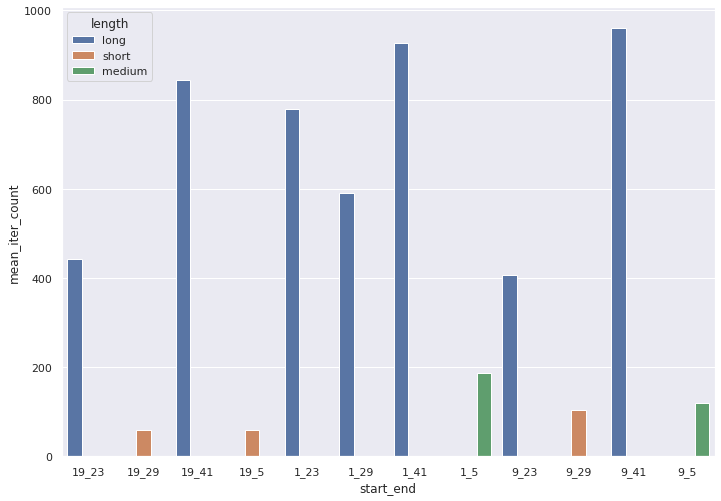
\includegraphics[scale=0.5]{images/se_iter_count.png}
\captionsetup{width=0.6\textwidth}
\caption{Mean iteration number depending on start/end configurations.}
\end{center}
\end{figure}

The pairs of points that BR-RRT struggled the most with were the ones, ending in point 41. The reason for this is that it is located in a very closed space, often making the algorithm getting stuck in narrow areas or exceeding iterations limit by exploring the whole map.

\end{document}